\section{Daganatos sejtek modellezése}
\begin{frame}
\frametitle{Daganatos sejtek modellezése}
\begin{itemize}
	\item daganat - sokszoros mutáció következtében létrejött elburjánzó sejttömörülés
	\item egy daganaton belül többféle sejt $\rightarrow$ agresszívabb sejttípusok megjelenése
\end{itemize}
	\begin{block}{}
	$\Rightarrow$ a játékelmélet egy lehetséges eszköz a sejttípusok közötti versengés modellezésére
\end{block}

\end{frame}

\begin{frame}
	\frametitle{Daganatos sejtek modellezése}
	Lehetséges modellek:
	\begin{itemize}
		\item daganatos sejtek - erőforrásokért folyatott \textbf{verseny}
		\item növekedési faktorokat termelő egészséges sejtek és daganatos sejtek - \textbf{parazitizmus}
		\item immunsejtek - \textbf{ragadozó}
		\item egészséges sejtek, daganatos sejtek - \textbf{mutualizmnus}
	\end{itemize}
\begin{figure}
	\centering
	\begin{tikzpicture}
	\node[anchor=south west,inner sep=0] (image) at (4,0) { 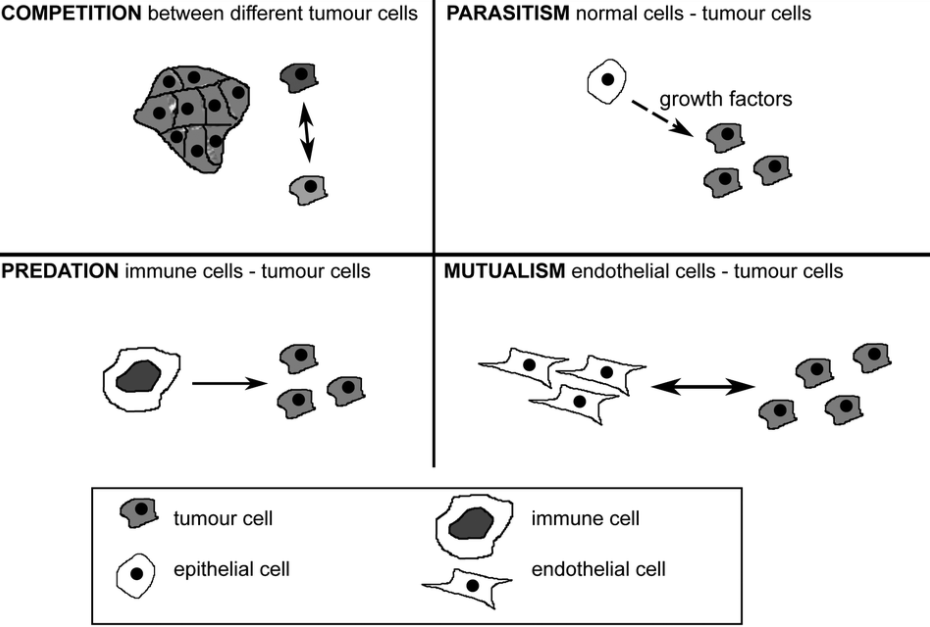
\includegraphics[width=0.5\linewidth]{images/models}};
	\pause
	\begin{scope}[x={(image.south east)},y={(image.north west)}]
	\draw[red,ultra thick,rounded corners] (0.15,0.6) rectangle (0.28,1);
	\end{scope}
	\end{tikzpicture}
\end{figure}
\end{frame}

\subsection{Közjó játék (Public goods game)}
\begin{frame}
\begin{itemize}
	\item növekedési faktorok és jelzőmolekulák szerepe
	\begin{itemize}
		\item saját növekedés elősegítése
		\item a szervezet védekezésének kijátszása
		\item metasztázis kialakulása
	\end{itemize}
	\item ezek az anyagok kikerülhetnek a sejtek közötti térbe
\end{itemize}
\begin{block}
	\centering
	$\Rightarrow$ növekedési faktor mint "közös jó"
\end{block}
\frametitle{Közjó játék (Public goods game)}\end{frame}

\subsection{A játékmodell felépítése}
\subsubsection{Voronoi diagram}
\begin{frame}
	\frametitle{Voronoi diagram}
	\begin{block}{}
		\begin{itemize}
			\item a sejtek ábrázolása Voronoi hálózatokkal
			\item \sout{szabályos pontrács}
			\item \sout{skála-független hálózatok}
		\end{itemize}
	\end{block}
	
	\centering
	
\includegraphics[width=0.5\linewidth]{images/Voronoi}
\end{frame}

\subsubsection{A játék szereplői és a stratégiák}
\begin{frame}
	\frametitle{A játék szereplői és a stratégiák}
	A sejtek:
	\begin{itemize}
		\item \textit{kooperálnak} - termelnek növekedési faktorokat
		\item \textit{defektálnak} - nem vesznek részt a faktorok termelésében
	\end{itemize}
	A stratégiák \textit{nyereségének (payoff)} kiszámítása: \(p = b(j) - c\)
	\begin{itemize}
		\item \textit{c} - a növekedési faktor előállításának költsége
		\item \textit{j} - a csoportban résztvevő kooperatív sejtek száma
	\end{itemize}
	ahol 
	\begin{equation}
		b(j) = [V(j) - V(0)]/[V(n) - V(0)]
	\end{equation}
	\begin{equation}
		\label{eq:payoffGradient}
		V(j) = 1/[1 + e^{(-s(j-k)/n)}]
	\end{equation}
\end{frame}

\begin{frame}
	\frametitle{Szabályok}
	\begin{itemize}
		\item véletlenszerűen elhelyezünk defektáló sejteket (arányuk 0.05)
		\item minden körben véletlenszerűen kiválasztunk egy sejtet és annak egy szomszédját 
		\item megvizsgáljuk a nyereségeket
		\item ha a szomszéd stratégiája kifizetődőbb, a kiválasztott sejt átveszi azt
		\item minden kör végén aktualizáljuk a nyereségeket (aszinkron módon számolunk)
	\end{itemize}
\end{frame}

\subsubsection{Diffúziós távolság}
\begin{frame}
	\frametitle{Diffúziós távolság}
	\begin{block}{}
		\begin{itemize}
			\item a diffúziós távolságon belül található összes sejt figyelembe vétele
			\item szomszédok befolyásának súlyozása - diffúziós gradiens
		\end{itemize}
		\begin{equation}
			\label{eq:diffGradient}
			G(i) = [g(i) - g(0)]/[g(D) - g(0)] 
		\end{equation}
		\begin{equation}
			g(i) = 1/[1 + e^{(-z(i-d)/D)}]
		\end{equation}
	\end{block}
	\begin{block}{}
		\begin{itemize}
				\item a termelők száma a \ref{eq:diffGradient}-sal kiszámított súlyozott összeg
		\end{itemize}
	\end{block}
\end{frame}

\subsection{Osztódás}
\begin{frame}
	\frametitle{Osztódás}
	\begin{block}{A Gompertz modell - a tumor méretének időbeli változása}
		\begin{equation}
			n_t = K \bigg(\frac{n_0}{K} \bigg) ^ {e^{(- \alpha t)}},
		\end{equation}
		\begin{itemize}
			\item $n_t$ - a populáció mérete a $t$ időpillanatban
			\item $n_0$ - a populáció kezdeti mérete
			\item $K$ - az elérhető maximális mérete a tumornak
			\item $\alpha$ - egy konstans, a sejtek burjánzási képességével áll összefüggésben
		\end{itemize}
	\end{block}
	\pause
	\begin{block}{}
		\begin{itemize}
			\item az eddigi modellbe könnyen beépíthető
			\item nem veszi figyelembe, hogy éppen milyen típusú sejt (kooperáló/defektáló) osztódik
		\end{itemize}
	\end{block}
\end{frame}